\section{\MSAGA{} Microarchitecture}


We implement \MSAGA{} in synthesizable RTL, using Chisel~\cite{chisel} as the hardware description language and Chipyard~\cite{chipyard,chipyard_dac,chipyard_iscas, cook2017diplomatic}
for system-on-chip (SoC) development.
Unlike prior efforts such as Gemmini~\cite{ucb-gemmini} that focus on
design space exploration, our objective is to provide a concrete and complete
implementation to evaluate both the feasibility of the
\SA{} kernel and the associated hardware cost of \MSAGA{}.

\subsection{Microarchitecture Overview}


\autoref{fig:msaga-microarchitecture} illustrates the microarchitecture of our \MSAGA{} accelerator.
\MSAGA{} receives instructions via an AXI4-Lite interface and accesses backing memory through
a configurable number of AXI4 memory interfaces. Received instructions are buffered in an instruction queue, decoded into
three types: \texttt{load}, \texttt{store}, and \texttt{compute}, and then dispatched
to the load queue, store queue, and systolic array controller, respectively.
Instructions of different types are executed asynchronously, while instructions of the same
type are issued in order with potential interleaving of their execution.

The systolic array controller issues compute instructions once the required data
has been loaded into SRAM. To simplify control logic, \MSAGA{} prioritizes SRAM
access over compute,
so that the latency of compute instructions becomes fully deterministic once issued.
This design allows the controller to statically schedule control signals
based on the progress of each instruction.

The DMA engine follows an iDMA-style interface~\cite{iDMA} and supports 2D data transfers.
Each \texttt{load} or \texttt{store} instruction can specify source and destination
addresses in SRAM and backing memory, along with the transfer size and stride.
When multiple AXI4 channels are available, the DMA engine automatically partitions the transfer
into parallel AXI4 transactions, maximizing memory bandwidth utilization.

\begin{figure}[t]
  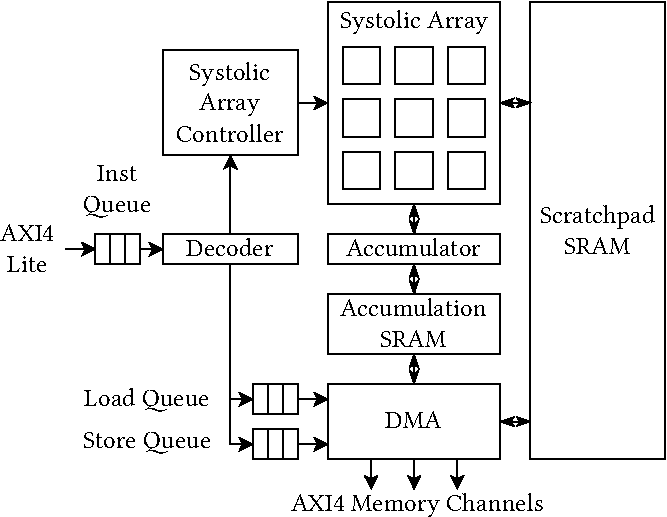
\includegraphics[scale=0.75]{figure_src/microarch.drawio.pdf}
  \caption{Microarchitecture of the \MSAGA{} accelerator.}
  \label{fig:msaga-microarchitecture}
  \Description{\MSAGA{} microarchitecture overview.}
\end{figure}


\subsection{\MSAGA{} Instruction Set}

To enable fine-grained overlap between various \FA{} operations, the 
systolic array in \MSAGA{} requires more sophisticated control logic 
than standard systolic arrays. The primary design goal of the \MSAGA{} 
instruction set is to ensure that \texttt{compute} instructions execute in a 
fully deterministic manner, independent of memory access latency,
which greatly reduces control complexity.

\begin{figure}[t]
  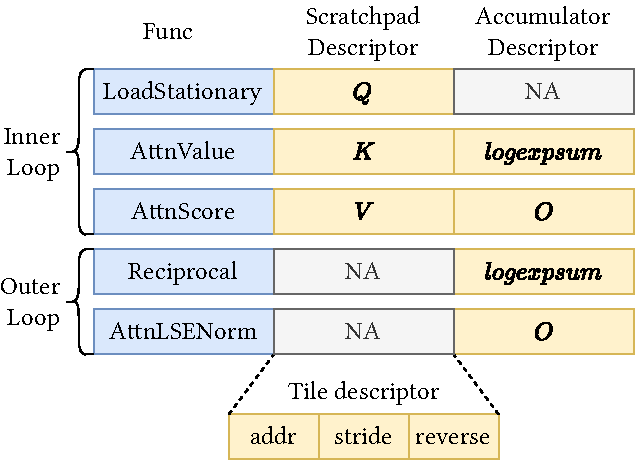
\includegraphics[scale=0.75]{figure_src/isa.drawio.pdf}
  \caption{\MSAGA{} compute instructions.}
  \label{fig:msaga-isa}
  \Description{\MSAGA{} compute instructions overview.}
\end{figure}

To this end, we define five compute instructions based on their SRAM 
data dependencies, as illustrated in 
\autoref{fig:msaga-isa}. The \FA{} inner loop is divided into 
three phases:

\begin{itemize}
  \item \texttt{LoadStationary}: preload $Q$ into the systolic array.
  \item \texttt{AttnScore}: perform the first matrix multiplication using 
  $Q$ and $K$, fused with element-wise online softmax to compute the 
  $P$ matrix in-place within the systolic array. The log of the exponent 
  sum for $P$ is also calculated during this step.
  \item \texttt{AttnValue}: perform the second matrix multiplication 
  using $V$ and $P$.
\end{itemize}

The \FA{} outer loop is divided into two additional phases:

\begin{itemize}
  \item \texttt{Reciprocal}: load the log exponent sum of $P$ from the 
  accumulation SRAM and compute its reciprocal. The result is stored 
  in the accumulator as a scaling factor for the next phase.
  \item \texttt{AttnLSENorm}: load the output matrix $O$ from the 
  accumulator and apply the reciprocal scaling factor.
\end{itemize}

Each compute instruction reads one input tile from SRAM and writes one 
output tile to the accumulator SRAM. This one-tile-in, one-tile-out 
design ensures that compute instructions can be executed as soon as 
their corresponding SRAM tile is ready, without waiting for other tiles 
to be loaded or processed.
DMA instructions follow a similar structure to compute instructions, 
consisting of one memory tile descriptor and one SRAM tile descriptor. 
However, they use wider bit fields to support large memory address 
spaces.

\subsection{Systolic Array Controller}

The microarchitecture of the systolic array controller is illustrated in \autoref{fig:msaga-controller}.
It mainly comprises two identical finite state machines (FSMs) for generating control signals to the systolic array and
the scratchpad/accumulator SRAM for the current and next \texttt{compute} instruction.
Each FSM contains a counter to track the progress of a \texttt{compute} instruction.
The counter is initialized at the start of the execution, incremented every cycle, and reset to zero upon completion.
As the execution of a \texttt{compute} instruction is fully deterministic,
the FSM simply generates all control signals solely based on the instruction type and the current counter value. 

The dual-FSM architecture of the systolic array controller enables 
efficient operation overlap, as described in \autoref{sec:overlapping-computations}. 
For example, the \texttt{AttnValue} instruction can begin execution 
as soon as the last \texttt{AttnScore} instruction produces the 
first element of the $P$ matrix. The \emph{combiner} unit merges control 
signals from both FSMs, ensuring that all signals are emitted in 
the correct order without conflict.


\begin{figure}[t]
  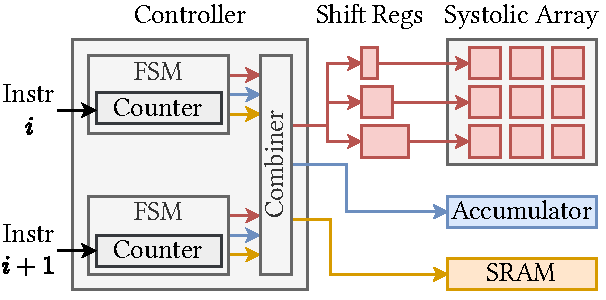
\includegraphics[scale=0.75]{figure_src/controller.drawio.pdf}
  \caption{\MSAGA{} systolic array controller.}
  \label{fig:msaga-controller}
  \Description{\MSAGA{} controller overview.}
\end{figure}

\begin{figure}[t]
  \centering
  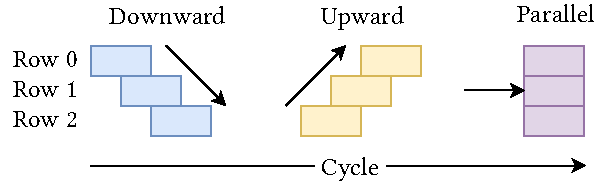
\includegraphics[scale=0.75]{figure_src/dsl.drawio.pdf}
  \caption{Three PE control flow propagation patterns in the systolic array: 
  Downward, Upward, and Parallel.}
  \label{fig:msaga-dsl}
  \Description{Three PE control flow propagation patterns in the systolic array.}
\end{figure}

There are three control flow propagation patterns in the systolic array: 
\emph{downward}, \emph{upward}, and \emph{parallel}, as illustrated in 
\autoref{fig:msaga-dsl}. The downward pattern propagates control signals 
from the top row to the bottom row; the upward pattern does the reverse; 
and the parallel pattern sends control signals to all rows simultaneously.
The control signals for downward and upward patterns can be generated 
using shift registers without duplicating control logic 
for each row. The parallel pattern can be implemented by broadcasting 
a single control signal to all rows.

To simplify control logic development, we implement a domain-specific 
language (DSL) on top of Chisel and Scala, as shown in \autoref{lst:dsl}. 
This DSL allows designers to specify which control signals should be 
scheduled at each clock cycle. The control logic is then automatically 
synthesized from the DSL specification.

\begin{listing}
\begin{mintedscala}
class PEControl {
  def parallel(start: Int, duration: Int) = ...
  def upward(start: Int, duration: Int) = ...
  def downward(start: Int, duration: Int) = ...
}
class ExampleInstruction(rows: Int, cols: Int)
  extends ExecutionPlan {
  // Load input tile into each row in parallel
  // from cycle 1 to 1 + cols
  load_reg.parallel(1, cols)
  ...
  // Perform MAC operation bottom-up using the
  // upward data path
  mac.upward(1 + cols, rows)
  ...
  // Perform MAC operation top-down using the
  // downward data path
  mac.downward(1 + cols + rows, rows)
}
\end{mintedscala}
\caption{\MSAGA{} Controller DSL.}
\label{lst:dsl}
\end{listing}
